\documentclass[border=10pt]{standalone}
\usepackage{pgfplots}
\usepgfplotslibrary{colormaps}
\pgfplotsset{compat=1.18}

\begin{document}
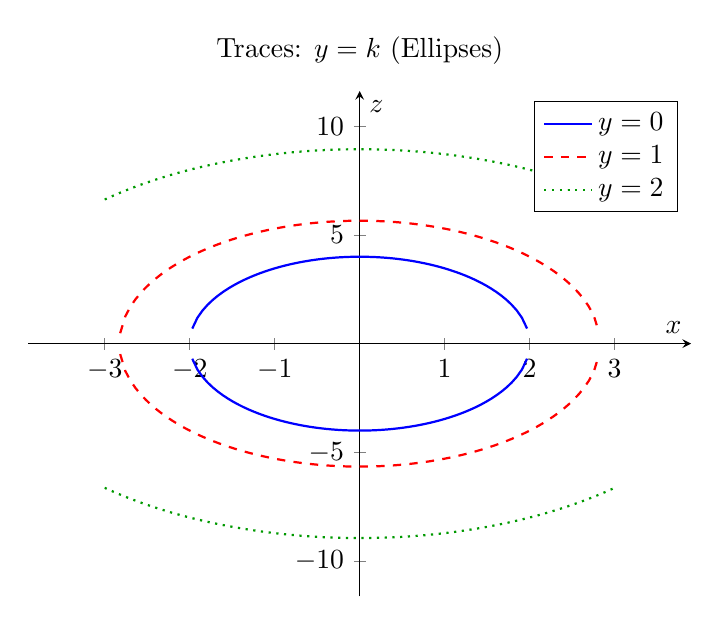
\begin{tikzpicture}
\begin{axis}[
    xlabel=$x$,
    ylabel=$z$,
    title={Traces: $y = k$ (Ellipses)},
    width=10cm,
    height=8cm,
    axis lines=center,
    enlargelimits=0.15,
    samples=100,
    domain=-3:3,
]
\addplot[blue, thick] {sqrt(16 - 4*x^2)};
\addplot[blue, thick] {-sqrt(16 - 4*x^2)};
\addplot[red, thick, dashed] {sqrt(32 - 4*x^2)};
\addplot[red, thick, dashed] {-sqrt(32 - 4*x^2)};
\addplot[green!60!black, thick, dotted] {sqrt(80 - 4*x^2)};
\addplot[green!60!black, thick, dotted] {-sqrt(80 - 4*x^2)};
\legend{$y=0$, , $y=1$, , $y=2$, }
\end{axis}
\end{tikzpicture}
\end{document}
